\documentclass[12pt]{article}

\setlength{\topmargin}{-.75in} \addtolength{\textheight}{2.00in}
\setlength{\oddsidemargin}{.00in} \addtolength{\textwidth}{.75in}

\usepackage{amsmath,color,graphicx}
\usepackage{enumerate}
\nofiles

\pagestyle{empty}

\setlength{\parindent}{0in}


\begin{document}

\noindent {\sc {\bf {\Large Final Exam}}
            \hfill SABIC Physics, Winter 2016}
\bigskip

\noindent {\sc  {}
            \hfill {\large Name:}
             \hfill}
\bigskip

{\bf Problem 1.}(12 points.) Short answer--no more than one sentence each. 
\begin{enumerate}[(a)]
\item If $\vec{C} = \vec{A} + \vec{B}$ and $|C| = |A| + |B|$, then what must be true about $\vec{A}$ and $\vec{B}$?
\bigskip
\bigskip
\bigskip
\bigskip
\bigskip
\item A dripping shower faucet releases drops at a rate of 10 per second (or one drop every $0.1$s). Find the seperation (difference in height) between two consecutive drops when (i) the topmost drop just leaves the faucet, and (ii) when the bottommost drop is $1$m below the faucet.
\bigskip
\bigskip
\bigskip
\bigskip
\bigskip
\bigskip
\bigskip
\bigskip
\bigskip
\item James Bond's Aston Martin strikes a henchman's BMW head on, and the henchman, not wearing his seatbelt, is thrown out of the front of his car. Use Newton's laws of motion to explain why this happens.
\bigskip
\bigskip
\bigskip
\bigskip
\bigskip
\bigskip
\bigskip
\item A force exerts total work $W$ to accelerate an object from rest to $10$m/s. In terms of $W$, how much work must be done to accelerate the object from that $10$m/s to $20$m/s? 
\bigskip
\bigskip
\bigskip
\bigskip
\bigskip
\item Two objects $A$ and $B$ are launched into the air using identical springs compressed by the same distance. The mass of object $A$ is twice the mass of object $B$. At its maximum height, object $B$ has a potential energy of $100$J. What is the gravitational potential energy of object $A$ at its own maximum height?
\bigskip
\bigskip
\bigskip
\bigskip
\bigskip
\end{enumerate}
\newpage
{\bf Problem 2.}(14 points.) (Motion in 2 dimensions):
A shell is fired with initial velocity $40$m/s at $60^\circ$ above the horizontal and feels no air resistance.
\begin{enumerate}[(a)]
\item Find the horizontal and vertical components of the initial velocity
\bigskip
\bigskip
\bigskip
\bigskip
\bigskip
\item Calculate the time it takes for the shell to reach its highest point.
\bigskip
\bigskip
\bigskip
\bigskip
\bigskip
\bigskip
\bigskip
\item Find the maximum height the shell reaches above the ground.
\bigskip
\bigskip
\bigskip
\bigskip
\bigskip
\bigskip
\bigskip
\item How far from the firing point does the shell land?
\bigskip
\bigskip
\bigskip
\bigskip
\bigskip
\bigskip
\bigskip
\item At its highest point, find the horizontal and vertical components of its acceleration and velocity.
\bigskip
\bigskip
\bigskip
\bigskip
\bigskip
\end{enumerate}
\newpage
{\bf Problem 3.}(14 points.) (Work and kinetic energy, Newton's Laws):
A $5.00$kg package slides $2.80$m down a long ramp inclined $24.0^\circ$ below the horizontal. The coefficient of kinetic friction between the package and the ramp is $\mu_k = 0.310$. 
\begin{enumerate}[(a)]
\item Draw a force diagram on the package, and label all forces.
\bigskip
\bigskip
\bigskip
\bigskip
\bigskip
\bigskip
\bigskip
\item Using Newton's Laws, calculate the acceleration on the package.
\bigskip
\bigskip
\bigskip
\bigskip
\bigskip
\bigskip
\bigskip
\item Calculate the work done by friction on the package.
\bigskip
\bigskip
\bigskip
\bigskip
\bigskip
\bigskip
\bigskip
\item Calculate the work done by gravity on the package.
\bigskip
\bigskip
\bigskip
\bigskip
\bigskip
\bigskip
\bigskip
\item What is the final velocity of the package after it slides the $2.80$m if the initial velocity was $2.20$m/s?
\bigskip
\bigskip
\bigskip
\end{enumerate}
\newpage
{\bf Problem 4.}() (Energy and motion in a circle)
A small block with a mass of $0.06$kg is attached to a cord passing through a hole in a frictionless, horizontal surface (see figure), which you hold with your hand. The block is originally revolving at a distance of $0.4$m from the holes with a speed of $0.70$m/s. 
\begin{figure}[!ht]
  \centering
    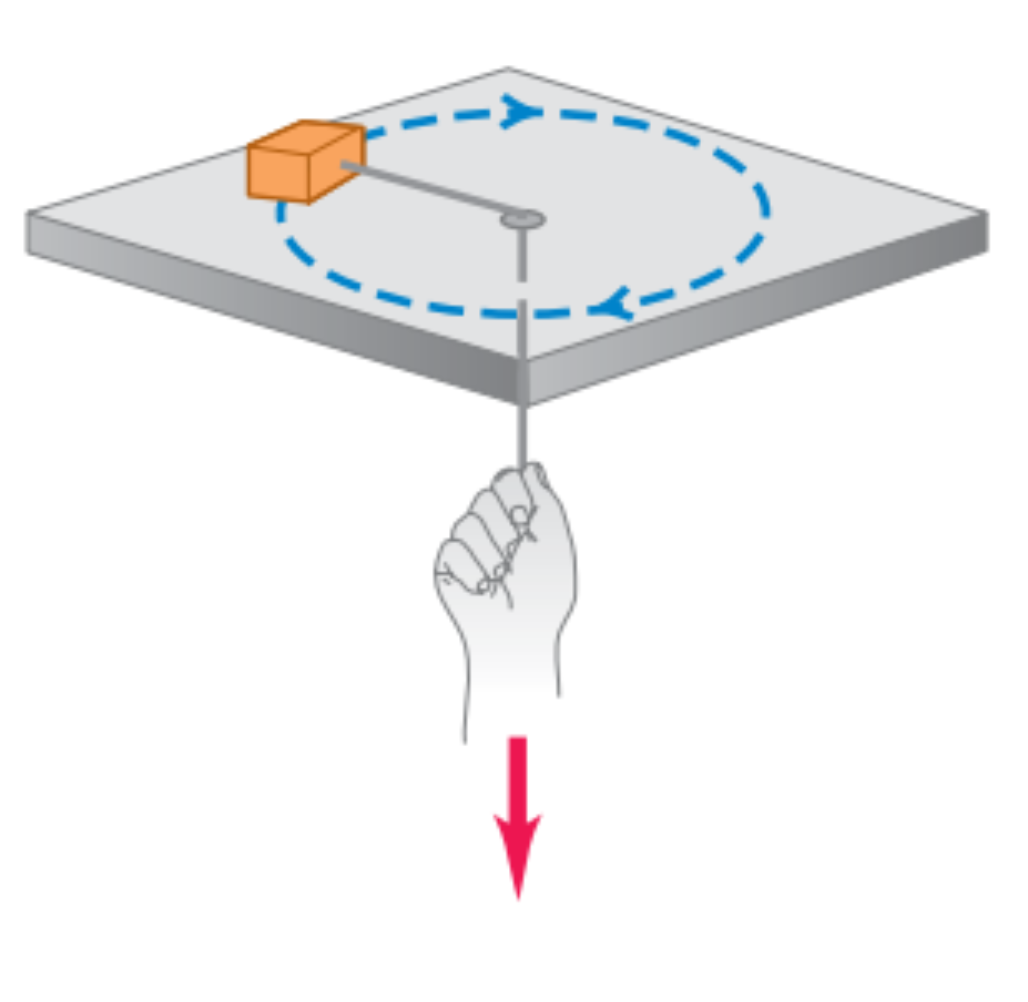
\includegraphics[width=0.5\textwidth]{figure1.png}
\end{figure}
\begin{enumerate}[(a)]
\item Calculate the tension on the string.
\bigskip
\bigskip
\bigskip
\bigskip
\bigskip
\item How much work is done by this tension force to keep the block revolving in a circle?
\bigskip
\bigskip
\bigskip
\bigskip
\bigskip
\item You then pull the string, shortening the radius of the circle in which the block revolves to $0.1$m, and increasing its speed to $2.8$m/s. Calculate the new tension of the cord.
\bigskip
\bigskip
\bigskip
\bigskip
\bigskip
\item How much work did you do to shorten the radius of the circle?
\bigskip
\bigskip
\bigskip
\bigskip
\bigskip
\item Calculate the average tension on the string during the time you shortened the circle. 
\bigskip
\bigskip
\bigskip
\bigskip
\bigskip
\end{enumerate}
\end{document}
